\documentclass{beamer}

\usepackage[T1]{fontenc}
\usepackage[utf8]{inputenc}
\usepackage[italian]{babel}
\usepackage{textcomp}
\usepackage{graphicx, amsmath, amssymb, listings, eurosym}
\usepackage{wrapfig}
\setbeamercolor*{alerted text}{fg=blue!80!black}
\usefonttheme{professionalfonts}
\usepackage{stmaryrd}
\lstset{
	mathescape,
	basicstyle=\scriptsize
}

\usetheme{Madrid}


\makeatother
\setbeamertemplate{footline}{
	\leavevmode%
	\hbox{%
		\begin{beamercolorbox}[wd=.25\paperwidth,ht=2.25ex,dp=1ex,center]{author in head/foot}\usebeamerfont{author in head/foot} {Colognese, Rossini}
		\end{beamercolorbox}%
		\begin{beamercolorbox}[wd=.6\paperwidth,ht=2.25ex,dp=1ex,center]{title in head/foot}%
			\usebeamerfont{title in head/foot}\insertshorttitle
	\end{beamercolorbox}}%
	\begin{beamercolorbox}[wd=.15\paperwidth,ht=2.25ex,dp=1ex,center]{date in head/foot}%
		\usebeamerfont{date in head/foot}
		\insertframenumber{} / \inserttotalframenumber
	\end{beamercolorbox}}%
	\vskip0pt%
\makeatletter

%%% Titolo e autore.
\title{Analisi dei Sistemi Informatici:\\ Dominio Astratto degli Intervalli}
\author{Marco Colognese \scriptsize VR423791 \\ \normalsize Mattia Rossini \scriptsize VR423614\normalsize}
\institute{Università degli Studi di Verona\\ \fontsize{2.3mm}{4mm} \selectfont Corso di Laurea Magistrale in Ingegneria e Scienze Informatiche}
\date{\newline \scriptsize Ottobre 2018\normalsize}



\begin{document}
	\begin{frame}
		\titlepage
	\end{frame}


\section[Sommario]{}
	\begin{frame}
		\tableofcontents
	\end{frame}


\section{Background}
	\begin{frame}
		\frametitle{Background}
		\framesubtitle{Analisi statica}
		L’\alert{analisi statica} permette di calcolare un'approssimazione dell'insieme dei valori o dei comportamenti che si verificheranno durante l'esecuzione di un programma senza avviarlo.
		
		\bigskip
		\alert{Approssimazione}: se denotiamo con \textlbrackdbl $\cdot$\textrbrackdbl\hspace{0.01cm} il comportamento concreto del programma e con \textlbrackdbl $\cdot$\textrbrackdbl\textsuperscript{$\sharp$} quello approssimato si ha che:
		\begin{center}
			\textlbrackdbl P\textrbrackdbl\hspace{0.01cm} $\subseteq$ \textlbrackdbl P\textrbrackdbl\textsuperscript{$\sharp$}
		\end{center}
	
		\bigskip
		Uno dei principali approcci dell'analisi statica è l'interpretazione astratta.
		
	\end{frame}

	\begin{frame}
		\frametitle{Background}
		\framesubtitle{Interpretazione Astratta}
		L’\alert{interpretazione astratta} è un framework per l'analisi statica che definisce un'astrazione corretta per la semantica concreta di un programma.
		
		\bigskip
		Per creare un'\alert{astrazione} occorre:
		\begin{itemize}
			\item un \textit{dominio concreto C}: è il punto di partenza;
			\item un \textit{dominio astratto A}: è un'approssimazione di \textit{C} e modella alcune proprietà dei calcoli concreti, tralasciando informazioni superflue;
			\item una \textit{funzione di astrazione}: $\alpha: C \rightarrow A$;
			\item eventualmente una \textit{funzione di concretizzazione}: $\gamma: A \rightarrow C$.
		\end{itemize}
	

	\end{frame}






\section{Dominio astratto degli Intervalli}
	\begin{frame}
		\frametitle{Dominio astratto degli Intervalli}
		\framesubtitle{Definizione}
		Il \alert{dominio astratto degli Intervalli} è un dominio numerico non relazionale in cui un insieme di interi viene approssimato dal più piccolo intervallo che li contiene ed è così definito:
		\begin{align*}
		\mathbb{I} = \{ [l, u] ~|~ l\in \mathbb{Z} \cup \{ -\infty \}, u\in \mathbb{Z} \cup \{ + \infty \}, l\leq u \}
		\end{align*}
		
		Questo dominio è un \alert{reticolo} completo ed in particolare:
		\begin{itemize}
			\item l'ordinamento $\sqsubseteq$ è tale che $[a, b] \sqsubseteq [c, d]$ solo se l'intervallo $[a, b]$ è interamente contenuto in $[c, d]$, cioè $a\geq c$ e $b\leq d$;
			\item l'elemento \textit{top} $\top$ è l'intervallo $[-\infty, \infty]$ che contiene tutti gli altri;
			\item l'elemento \textit{bottom} $\bot$ è l'insieme vuoto che non contiene elementi. 
		\end{itemize}
	

	
	

	\end{frame}

	\begin{frame}
		\frametitle{Dominio astratto degli Intervalli}
		\framesubtitle{Accelerazione della convergenza}
		Questo dominio non rispetta la \textit{ACC}, dunque non garantisce la terminazione: perciò viene introdotto il \alert{widening $\nabla$}.
		Funziona come segue:
		\begin{align*}
		\lbrack a, b \rbrack\ \nabla\ \lbrack c, d \rbrack = \lbrack e, f \rbrack \qquad \text{t.c.~~~~~~~~~~~~~~~~}\\
		e = 
		\begin{cases}
		-\infty &\text{ se } c < a \\
		a &\text{ altrimenti}
		\end{cases}
		~~~~~~~f = 
		\begin{cases}
		+\infty &\text{ se } b < d\\
		b &\text{ altrimenti }
		\end{cases}
		\end{align*}
		
		\medskip
		Utilizzando il widening può capitare di avere eccessive perdite di precisione, perciò viene introdotto il \alert{narrowing $\triangle$}.
		Funziona come segue:
		\begin{align*}
		\lbrack a, b \rbrack\ \triangle\ \lbrack c, d \rbrack = \lbrack e, f \rbrack \qquad \text{t.c.~~~~~~~~~~~~~~}\\
		e = 
		\begin{cases}
		c &\text{ se } a = -\infty \\
		a &\text{ altrimenti}
		\end{cases}
		~~~~~~~f = 
		\begin{cases}
		d &\text{ se } b = +\infty\\
		b &\text{ altrimenti }
		\end{cases}
		\end{align*}

		\end{frame}
	




\section{Implementazione}
	\begin{frame}[fragile]
		\frametitle{Implementazione}
		\framesubtitle{Libreria}
		La libreria implementata è composta dalle seguenti classi:
		\begin{itemize}
			\item \alert{\textit{AbstractInterval}}: classe astratta, rappresenta un intervallo generico;
			\item \alert{\textit{IntegerAbstractInterval}} e \alert{\textit{FloatingPointAbstractInterval}}: estendono \textit{AbstractInterval} per intervalli rispettivamente interi e a virgola mobile;
			\item \alert{\textit{Bound}}: rappresenta un \textit{bound} che compone un intervallo;
			\item \alert{\textit{Infinity}}: rappresenta un valore infinito con il relativo segno;
			\item \alert{\textit{UndefinedOperationException}}: rappresenta l'eccezione per le operazioni non definite ed estende la classe \textit{exception}.
		\end{itemize}
	\begin{figure}[H]
		\centering
		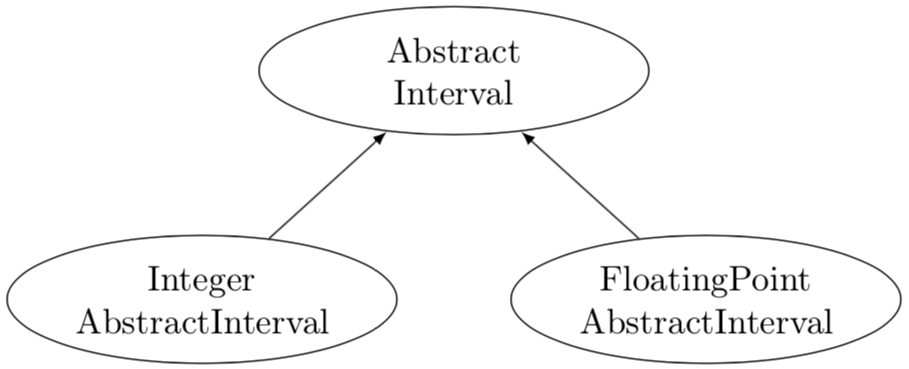
\includegraphics[scale=0.36]{pic}
	\end{figure}
\end{frame}


	\begin{frame}[fragile]			
		\frametitle{Implementazione}
		\framesubtitle{Linguaggio \textit{Toy}}
		Per provare la libreria, è stato definito un semplice linguaggio chiamato \alert{Toy}.\\
		\scriptsize
		\bigskip
		\hrule
\begin{lstlisting}
<program>	::= {<statement>\n}$^*$
<statement>	::= <assignment> | <conditional> | <loop>
<assignment>	::= <identifier> = <expression>
<conditional>	::= if <condition>\n {<assignment>\n}$^*$ endif
<loop>		::= while <condition>\n {<assignment>\n}$^*$ endwhile 
<expression>	::= <value> | <value> <operator> <value>
<value>		::= <identifier> | <number> | -<number>
<condition>	::= <identidier> <cmp> <number> | <boolean>
<boolean>	::= true | false
<operator>	::= + | - | * | / 
<identifier>	::= <letter> <id>$^*$
<cmp>		::= <= | >= | < | >
<id>		::= <letter> | <digit>
<number>	::= <digit>$^+$ | <digit>$^+$.<digit>$^+$
<letter>	::= a | b | ... | z | A | B | ... | Z
<digit>		::= 0 | 1 | 2 | 3 | 4 | 5 | 6 | 7 | 8 | 9
\end{lstlisting}
\hrule
\normalsize
\end{frame}

	\begin{frame}[fragile]
		\frametitle{Implementazione}
		\framesubtitle{Interprete per il linguaggio}
		L'interprete esegue in modo ordinato le seguenti fasi:
		\begin{enumerate}
			\item \alert{cerca} il programma nel file \textit{input.txt};
			\item \alert{legge} il file riga per riga, riconoscendo lo \alert{statement} di ognuno: assegnamento, \textit{if} oppure \textit{while};
			\item partendo dai valori delle variabili, genera i rispettivi \alert{intervalli};
			\item modifica gli intervalli attraverso le \alert{operazioni} della libreria;
			\item \alert{stampa} a video gli intervalli relativi a ciascuna variabile indicandone nome, \textit{lower bound} e \textit{upper bound}.
		\end{enumerate}	
\end{frame}

	\begin{frame}[fragile]
		\frametitle{Implementazione}
		\framesubtitle{Test}
		Per ogni classe è stato scritto un file di \alert{test}, basandosi sulla libreria \textit{Catch2}.
	
		\bigskip
		L'obiettivo è quello di fornire una \alert{copertura} del codice il più vicino possibile al $100\%$.
		Questi sono stati utili per verificare la corretta implementazione della libreria anche nei casi limite delle operazioni tra intervalli.

		\bigskip
		Per compilare ed avviare i test eseguire i seguenti comandi:
		\begin{itemize}
			\item \verb|make| (per compilare il codice);
			\item \verb|make test| (per eseguire i test).
		\end{itemize}

\end{frame}

	\begin{frame}[fragile]
		\frametitle{Implementazione}
		\framesubtitle{Documentazione}
		È stata scritta la \alert{documentazione} attraverso lo standard tool \textit{Doxygen}:
		\begin{itemize}
			\item per ogni \alert{funzione} vengono definiti una breve descrizione (\verb|@brief|), i parametri di input (\verb|@param|) ed il valore di ritorno (\verb|@return|);
			\item per ogni \alert{classe} viene definita una breve descrizione (\verb|@brief|);
			\item per ogni \alert{file} vengono definiti il copyright (\verb|@copyright|), la licenza (\verb|@license|), gli autori (\verb|@authors|), la data di produzione (\verb|@date|) e la versione del progetto (\verb|@version|).
		\end{itemize}

		\medskip
		Per generare la documentazione eseguire i seguenti comandi:
		\begin{itemize}
			\item \verb|make| (per compilare il codice);
			\item \verb|make doc| (per generare la documentazione).
		\end{itemize}
		Questa viene generata nella directory \textit{/doc} in formato \textit{HTML}.

\end{frame}





\section{Conclusioni}
	\begin{frame}
		\frametitle{Conclusioni}
		Sviluppare questo progetto ci ha permesso principalmente di:
		\begin{itemize}
			\item imparare il linguaggio \textit{C++};
			\item approfondire a fondo l'analisi statica, l'interpretazione astratta e, soprattutto, il dominio degli Intervalli;
			\item implementare e successivamente osservare il comportamento ed il funzionamento di tale dominio in ambito pratico;
			\item mettere in pratica le conoscenze teoriche acquisite durante il percorso di studi triennale, ovvero creare un interprete, organizzare il codice in classi e documentarlo per migliorarne la leggibilità.
		\end{itemize}


\end{frame}

\end{document}